\documentclass{article}

\usepackage{arxiv}

\usepackage[utf8]{inputenc} % allow utf-8 input
\usepackage[T1]{fontenc}    % use 8-bit T1 fonts
\usepackage{lmodern}        % https://github.com/rstudio/rticles/issues/343
\usepackage{hyperref}       % hyperlinks
\usepackage{url}            % simple URL typesetting
\usepackage{booktabs}       % professional-quality tables
\usepackage{amsfonts}       % blackboard math symbols
\usepackage{nicefrac}       % compact symbols for 1/2, etc.
\usepackage{microtype}      % microtypography
\usepackage{lipsum}
\usepackage{graphicx}

\title{Continuous risk-based predictive approaches to treatment effect
heterogeneity: A simulation study}

\author{
    Alexandros Rekkas
   \\
    Department of Medical Informatics \\
    Erasmus Medical Center \\
  Rotterdam, The Netherlands \\
  \texttt{} \\
   \And
    Peter R. Rijnbeek
   \\
    Department of Medical Informatics \\
    Erasmus Medical Center \\
  Rotterdam, The Netherlands \\
  \texttt{} \\
   \And
    Ewout W. Steyerberg
   \\
    Department of Biomedical Data Sciences \\
    Leiden University Medical Center \\
  Leiden, The Netherlands \\
  \texttt{} \\
   \And
    David van Klaveren
   \\
    Department of Public Health \\
    Erasmus Medical Center \\
  Rotterdam, The Netherlands \\
  \texttt{} \\
  }


% Pandoc citation processing
\newlength{\csllabelwidth}
\setlength{\csllabelwidth}{3em}
\newlength{\cslhangindent}
\setlength{\cslhangindent}{1.5em}
% for Pandoc 2.8 to 2.10.1
\newenvironment{cslreferences}%
  {}%
  {\par}
% For Pandoc 2.11+
\newenvironment{CSLReferences}[3] % #1 hanging-ident, #2 entry spacing
 {% don't indent paragraphs
  \setlength{\parindent}{0pt}
  % turn on hanging indent if param 1 is 1
  \ifodd #1 \everypar{\setlength{\hangindent}{\cslhangindent}}\ignorespaces\fi
  % set entry spacing
  \ifnum #2 > 0
  \setlength{\parskip}{#2\baselineskip}
  \fi
 }%
 {}
\usepackage{calc} % for calculating minipage widths
\newcommand{\CSLBlock}[1]{#1\hfill\break}
\newcommand{\CSLLeftMargin}[1]{\parbox[t]{\csllabelwidth}{#1}}
\newcommand{\CSLRightInline}[1]{\parbox[t]{\linewidth - \csllabelwidth}{#1}}
\newcommand{\CSLIndent}[1]{\hspace{\cslhangindent}#1}

\renewcommand*\familydefault{\sfdefault}
\usepackage{setspace}
\usepackage{amsmath}
\doublespacing
\usepackage[left]{lineno}
\usepackage{amssymb}
\usepackage{bm}
\usepackage{booktabs}
\newcommand\given[1][]{\:#1\vert\:}
\date{}
\usepackage{booktabs}
\usepackage{longtable}
\usepackage{array}
\usepackage{multirow}
\usepackage{wrapfig}
\usepackage{float}
\usepackage{colortbl}
\usepackage{pdflscape}
\usepackage{tabu}
\usepackage{threeparttable}
\usepackage{threeparttablex}
\usepackage[normalem]{ulem}
\usepackage{makecell}
\usepackage{xcolor}


\begin{document}
\maketitle

\def\tightlist{}


\begin{abstract}
\textbf{Objective:} Baseline risk is an important determinant of the
absolute effect of a treatment for an individual patient. We aimed to
compare different risk-based methods for predicting individualized
treatment effects with simulations of the RCT setting. \textbf{Study
Design} and Setting: We sampled patients from a superpopulation with
diverse assumptions for a baseline prognostic index of risk (PI), and
for the shape of the interaction between the PI and treatment (no,
linear or quadratic interaction). In each sample, we fitted different
models for predicting absolute benefit: a model with the PI and a
constant relative treatment effect and models including an interaction
of treatment assignment with the PI, with 4 quarters of the PI, and with
nonlinear transformations of the PI (restricted cubic splines with 3, 4
and 5 knots). We also used an adaptive model selection approach based on
Akaike's Information Criterion. We evaluated predictive performance in
the superpopulation using root mean squared error and measures of
discrimination and calibration for benefit. Starting from a base case
scenario (sample size 4,250, treatment odds ratio 0.8, AUC of the PI
0.75), we varied the sample size, the strength of the treatment effect,
and the discriminative ability of the PI. \textbf{Results:} Models
including a linear interaction of the PI with treatment had (close to?)
optimal performance under most simulation scenarios. More flexible
models with restricted cubic splines required larger sample sizes and
higher AUC of the PI to outperform the linear model. The adaptive
approach performed similarly to the best-performing method in each
scenario. \textbf{Conclusion:} Under most circumstances, a model with a
linear interaction of the PI with treatment is better able to predict
absolute treatment benefit.
\end{abstract}

\keywords{
    treatment effect heterogeneity
   \and
    absolute benefit
   \and
    prediction models
  }

\linenumbers

\hypertarget{introduction}{%
\section{Introduction}\label{introduction}}

Predictive approaches for assessing heterogeneity of treatment effects
(HTE) aim at the development of models predicting either individualized
effects or which of two (or more) treatments is better for an individual
{[}1{]}. In prior work, we divided such methods in three broader
categories based on the reference class used for defining patient
similarity when making individualized predictions or recommendations
{[}2{]}. Risk-modeling approaches use prediction of baseline risk as the
reference; treatment effect modeling approaches also model
treatment-covariate interactions, in addition to risk factors; optimal
treatment regime approaches focus on developing treatment assignment
rules and therefore rely heavily on modeling treatment effect modifiers.

Risk-modeling approaches to predictive HTE analyses provide a viable
option in the absence of well-established treatment effect modifiers
{[}3,4{]}. In simulations, modeling of effect modifiers, i.e.
treatment-covariate interactions, often led to miscalibrated predictions
of benefit, while risk-based methods proved quite robust {[}5{]}. Most
often, risk-modeling approaches are carried out in two steps: first a
risk prediction model is developed externally or internally on the
entire RCT population, ``blinded'' to treatment; then the RCT population
is stratified using this prediction model to evaluate risk-based
treatment effect variation {[}6{]}. However, even though estimates at
the risk subgroup level may be accurate, these estimated do not apply to
individual patients, especially for patients with predicted risk at the
boundaries of the risk intervals. Hence, the risk-stratified approach is
useful for exploring and presenting HTE, but is not useful for
supporting treatment decisions for individual patients.

To individualize treatment effects, the recent PATH statement suggested
various risk-based models including a prognostic index of baseline risk
(PI) and treatment assignment {[}cite PATH !!{]}. We aimed to summarize
and compare different risk-based models for predicting individualized
treatment effects. We simulated RCT settings to compare the performance
of these models under different assumptions of the relationship between
baseline risk and treatment. We illustrated the different models by a
case study of predicting individualized effects of tissue plasminogen
activator (tPA) versus streptokinase treatment in patients with an acute
myocardial infarction (MI).

\hypertarget{methods}{%
\section{Methods}\label{methods}}

\hypertarget{simulation-scenarios}{%
\subsection{Simulation scenarios}\label{simulation-scenarios}}

In the simulated datasets based treatment was allocated at random using
a 50:50 split. For each patient we simulated \(8\) baseline covariates,
where \(x_1,\dots,x_4\sim N(0, 1)\) and \(x_5,\dots,x_8\sim B(1, 0.2)\).
Outcomes for patients in the control arm were generated from a logistic
regression model including all baseline covariates. Coefficient values
were such, so that the prediction model had an AUC of \(0.75\) and an
event rate of \(20\%\) in the control arm was achieved. Under the base
case scenario, outcomes in the treatment arm were created using the same
logistic regression model, including a constant treatment odds ratio
(OR) of \(0.8\). The generated samples of the base case scenario had
sample size of 4,250 (\(85%
\) power for the detection of an unadjusted OR of \(0.8\)).

We evaluated the effect of sample size considering additional scenarios
with sample sizes of 1,064 and 17,000. We also evaluated the effect of
prediction performance, adjusting the baseline covariate coefficients,
so that AUC values of \(0.65\) and \(0.80\) were achieved when
validating in a simulated dataset of 500,000 patients.

We simulated binary outcomes in the control arm using true probabilities
\(P(y=1|X) = \text{expit}(PI)\), where
\(\text{expit}(x)= \frac{e^x}{1 + e^x}\). In the treatment arm outcomes
where generated with probabilities \(\text{expit}(lp_1)\) with
\[ lp_1 = \gamma_2(PI-c)^2 + \gamma_1(PI-c) + \gamma_0,\] where the
coefficients \(\gamma_0, \gamma_1\) and \(\gamma_2\) along with the
centering constant \(c\) were set for each simulation scenario. In this
way we were able to assess a wide variety of scenarios, ranging from
true constant relative treatment effects to moderate and strong linear
and quadratic deviations. We also considered scenarios with
treatment-covariate interactions. These scenarios include 4 weak
interactions (\(\text{OR}_{t_x=1} / \text{OR}_{t_x=0}=0.82\)), 4 strong
interactions (\(\text{OR}_{t_x=1} / \text{OR}_{t_x=0}=0.61\)), and 2
weak and 2 strong interactions. Combining all these different settings
resulted in a simulation study of \(66\) scenarios. The exact settings
for each scenario are available in the supplementary material.

\hypertarget{individualized-risk-based-benefit-predictions}{%
\subsection{Individualized risk-based benefit
predictions}\label{individualized-risk-based-benefit-predictions}}

All methods assume that a risk prediction model is available and can be
used to assign individualized risk predictions. For the simulations we
developed the prediction models internally and blinded to treatment
using logistic regression including main effects for all baseline
covariates and treatment. Risk predictions on individuals were made
setting treatment to \(0\).

The \emph{stratified HTE method} has been suggested as an alternative to
traditional subgroup analyses. Patients are stratified into
equally-sized risk strata---in this case based on risk quartiles.
Absolute effects are estimated using the differences in event rates
between treatments within risk quarters. We considered this approach as
a reference, expecting it to perform worse than the other candidates, as
its objective is not individualized benefit prediction.

Another approach would be to assume \emph{constant relative treatment
effect} (OR) is constant. In that case, absolute benefit is estimated
from \(\hat{\tau}(\bm{x}) = \text{expit}(PI +\log(\text{OR}))\), where
\(\text{expit}(x)=\frac{e^x}{1+e^x}\) and \emph{lp} is the linear
predictor of the prediction model.

A different approach fits a logistic regression using treatment, the
prognostic index and their interaction. In this case absolute benefit is
estimated from
\(\text{expit}(\beta_0+\beta_{PI}PI) - \text{expit}(\beta_0+\beta_{t_x}+(\beta_{PI}+\beta_*)PI)\).
We will refer to this method as the \emph{linear interaction} approach.

Finally, we used \emph{restricted cubic splines} (RCS) to relax the
linearity assumption on the effect of the linear predictor {[}7{]}. We
compared the results for 3, 4 and 5 knots when fitting the splines to
introduce increasing flexibility to the methods considered.

\hypertarget{evaluation-metrics}{%
\subsection{Evaluation metrics}\label{evaluation-metrics}}

For evaluating the prediction error of the considered methods we used
root mean squared error (RMSE), since both the true and the predicted
benefits are known, given that this is a simulation study. More
specifically, we calculated RMSE from
\[\text{RMSE}=\frac{1}{n}\sum_{i=1}^n\big(\tau(\bm{x}_i) - \hat{\tau}(\bm{x}_i)\big)^2\]

We also compared the discriminative ability of the methods under study.
We assessed discrimination using the c-for-benefit statistic described
in {[}8{]}. Patients in each treatment arm are ranked based on their
predicted benefit and then are matched 1:1, dropping patients in the
larger treatment arm without a pair. We define \emph{observed}
pair-specific treatment benefit as the difference of observed outcomes
between the untreated and the treated patient of each pair.
Pair-specific \emph{predicted} benefit is defined as the average of
predicted benefits within each pair. Then, c-for-benefit is defined as
the probability that from two randomly chosen matched patient pairs with
unequal observed benefit, the pair with greater observed benefit also
has a higher predicted benefit.

We evaluated calibration in a similar manner, using the integrated
calibration index (ICI) for benefit {[}9{]}. After creating pairs based
on predicted benefit, observed benefits are regressed on the predicted
benefits using a locally weighted scatterplot smoother (loess). The ICI
is the average absolute difference between predicted and smooth observed
benefit. Values closer to \(0\) represent better calibration.

\hypertarget{results}{%
\section{Results}\label{results}}

\hypertarget{simulations}{%
\subsection{Simulations}\label{simulations}}

The model including a constant relative treatment effect had the lowest
median RMSE in scenarios with a true constant relative treatment effect
(OR = 0.8, N = 4,250 and AUC = 0.75) or moderate relative deviations
were considered (Figure \ref{fig:rmsebase}; Panel A). However, when we
considered strong linear and quadratic deviations from a constant
relative treatment effect the linear interaction model performed best
(Figure \ref{fig:rmsebase}; Panels B and C). Only in the case of strong
quadratic deviations models including RCS (3 knots) performed equally
well to the linear interaction method. Increasing the number of knots in
RCS resulted in higher error rates across all scenarios. The adaptive
approach performed very similarly to the best performing model in each
scenario.

\begin{figure}
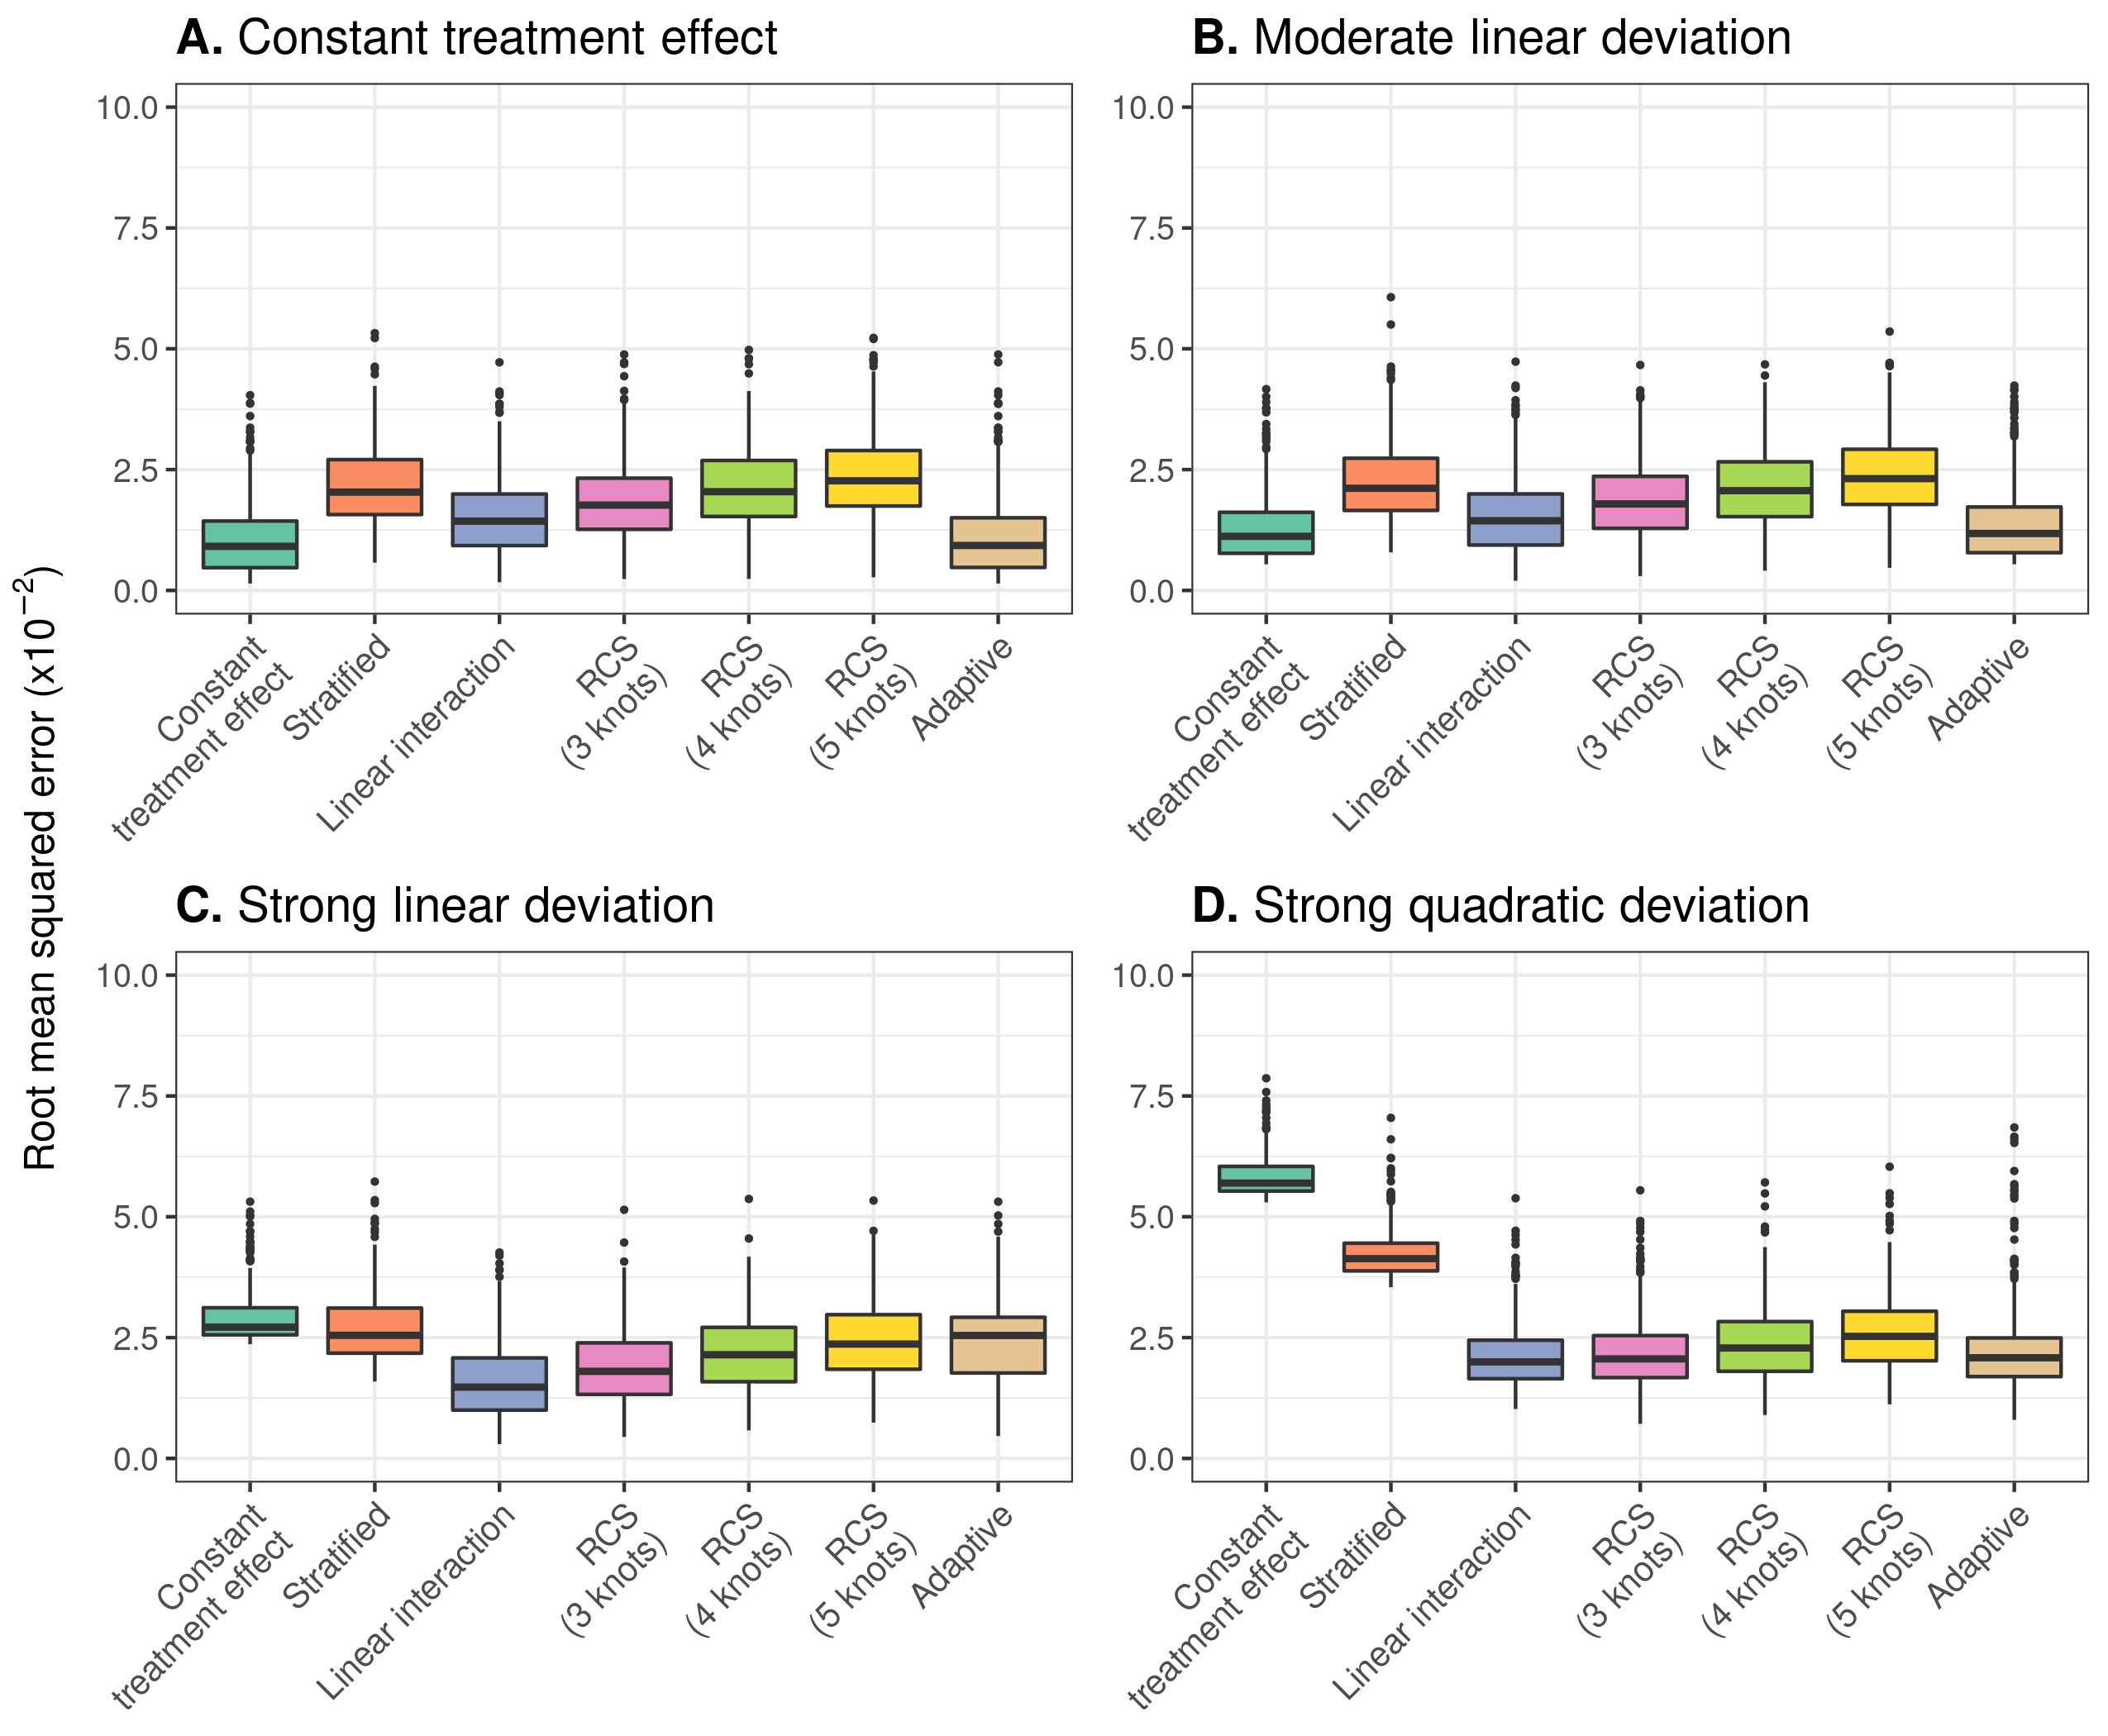
\includegraphics[width=1\linewidth]{/home/arekkas/Documents/Projects/arekkas_HteSimulation_XXXX_2021/figures/rmse_base} \caption{RMSE of the considered methods across 500 replications calculated in a simulated superpopulation of size 500,000. \textit{Panel A} presents the results of the scenario with true constant relative treatment effect, with a true prediction AUC of 0.75 and sample size of 4250; \textit{Panel B} presents the results under moderate linear deviations from constant treatment effects; \textit{Panel C} presents the results for strong linear deviations from constant relative treatment effects; \textit{Panel D} presents the results for strong quadratic deviations from constant relative treatment effects.}\label{fig:rmsebase}
\end{figure}

When we increased the sample size (N = 17,000), the model including a
constant relative treatment effect had the lowest RMSE under the
assumption of true constant relative treatment effects (Figure
\ref{fig:rmsesamplesize}; Panel A). Contrary to previous results with
smaller sample sizes, when introducing moderate and strong linear
deviations the linear interaction model performed best, outperforming
the constant treatment effect model (Figure \ref{fig:rmsesamplesize};
Panels B and C). However, the linear interaction model was outperformed
by the more flexible RCS models (3 knots) in the case of strong
quadratic deviations. Again, the increased flexibility of RCS smoothing
with higher number of knots resulted in overfitting and worse
performance (Figure \ref{fig:rmsesamplesize}; Panel D).

\begin{figure}
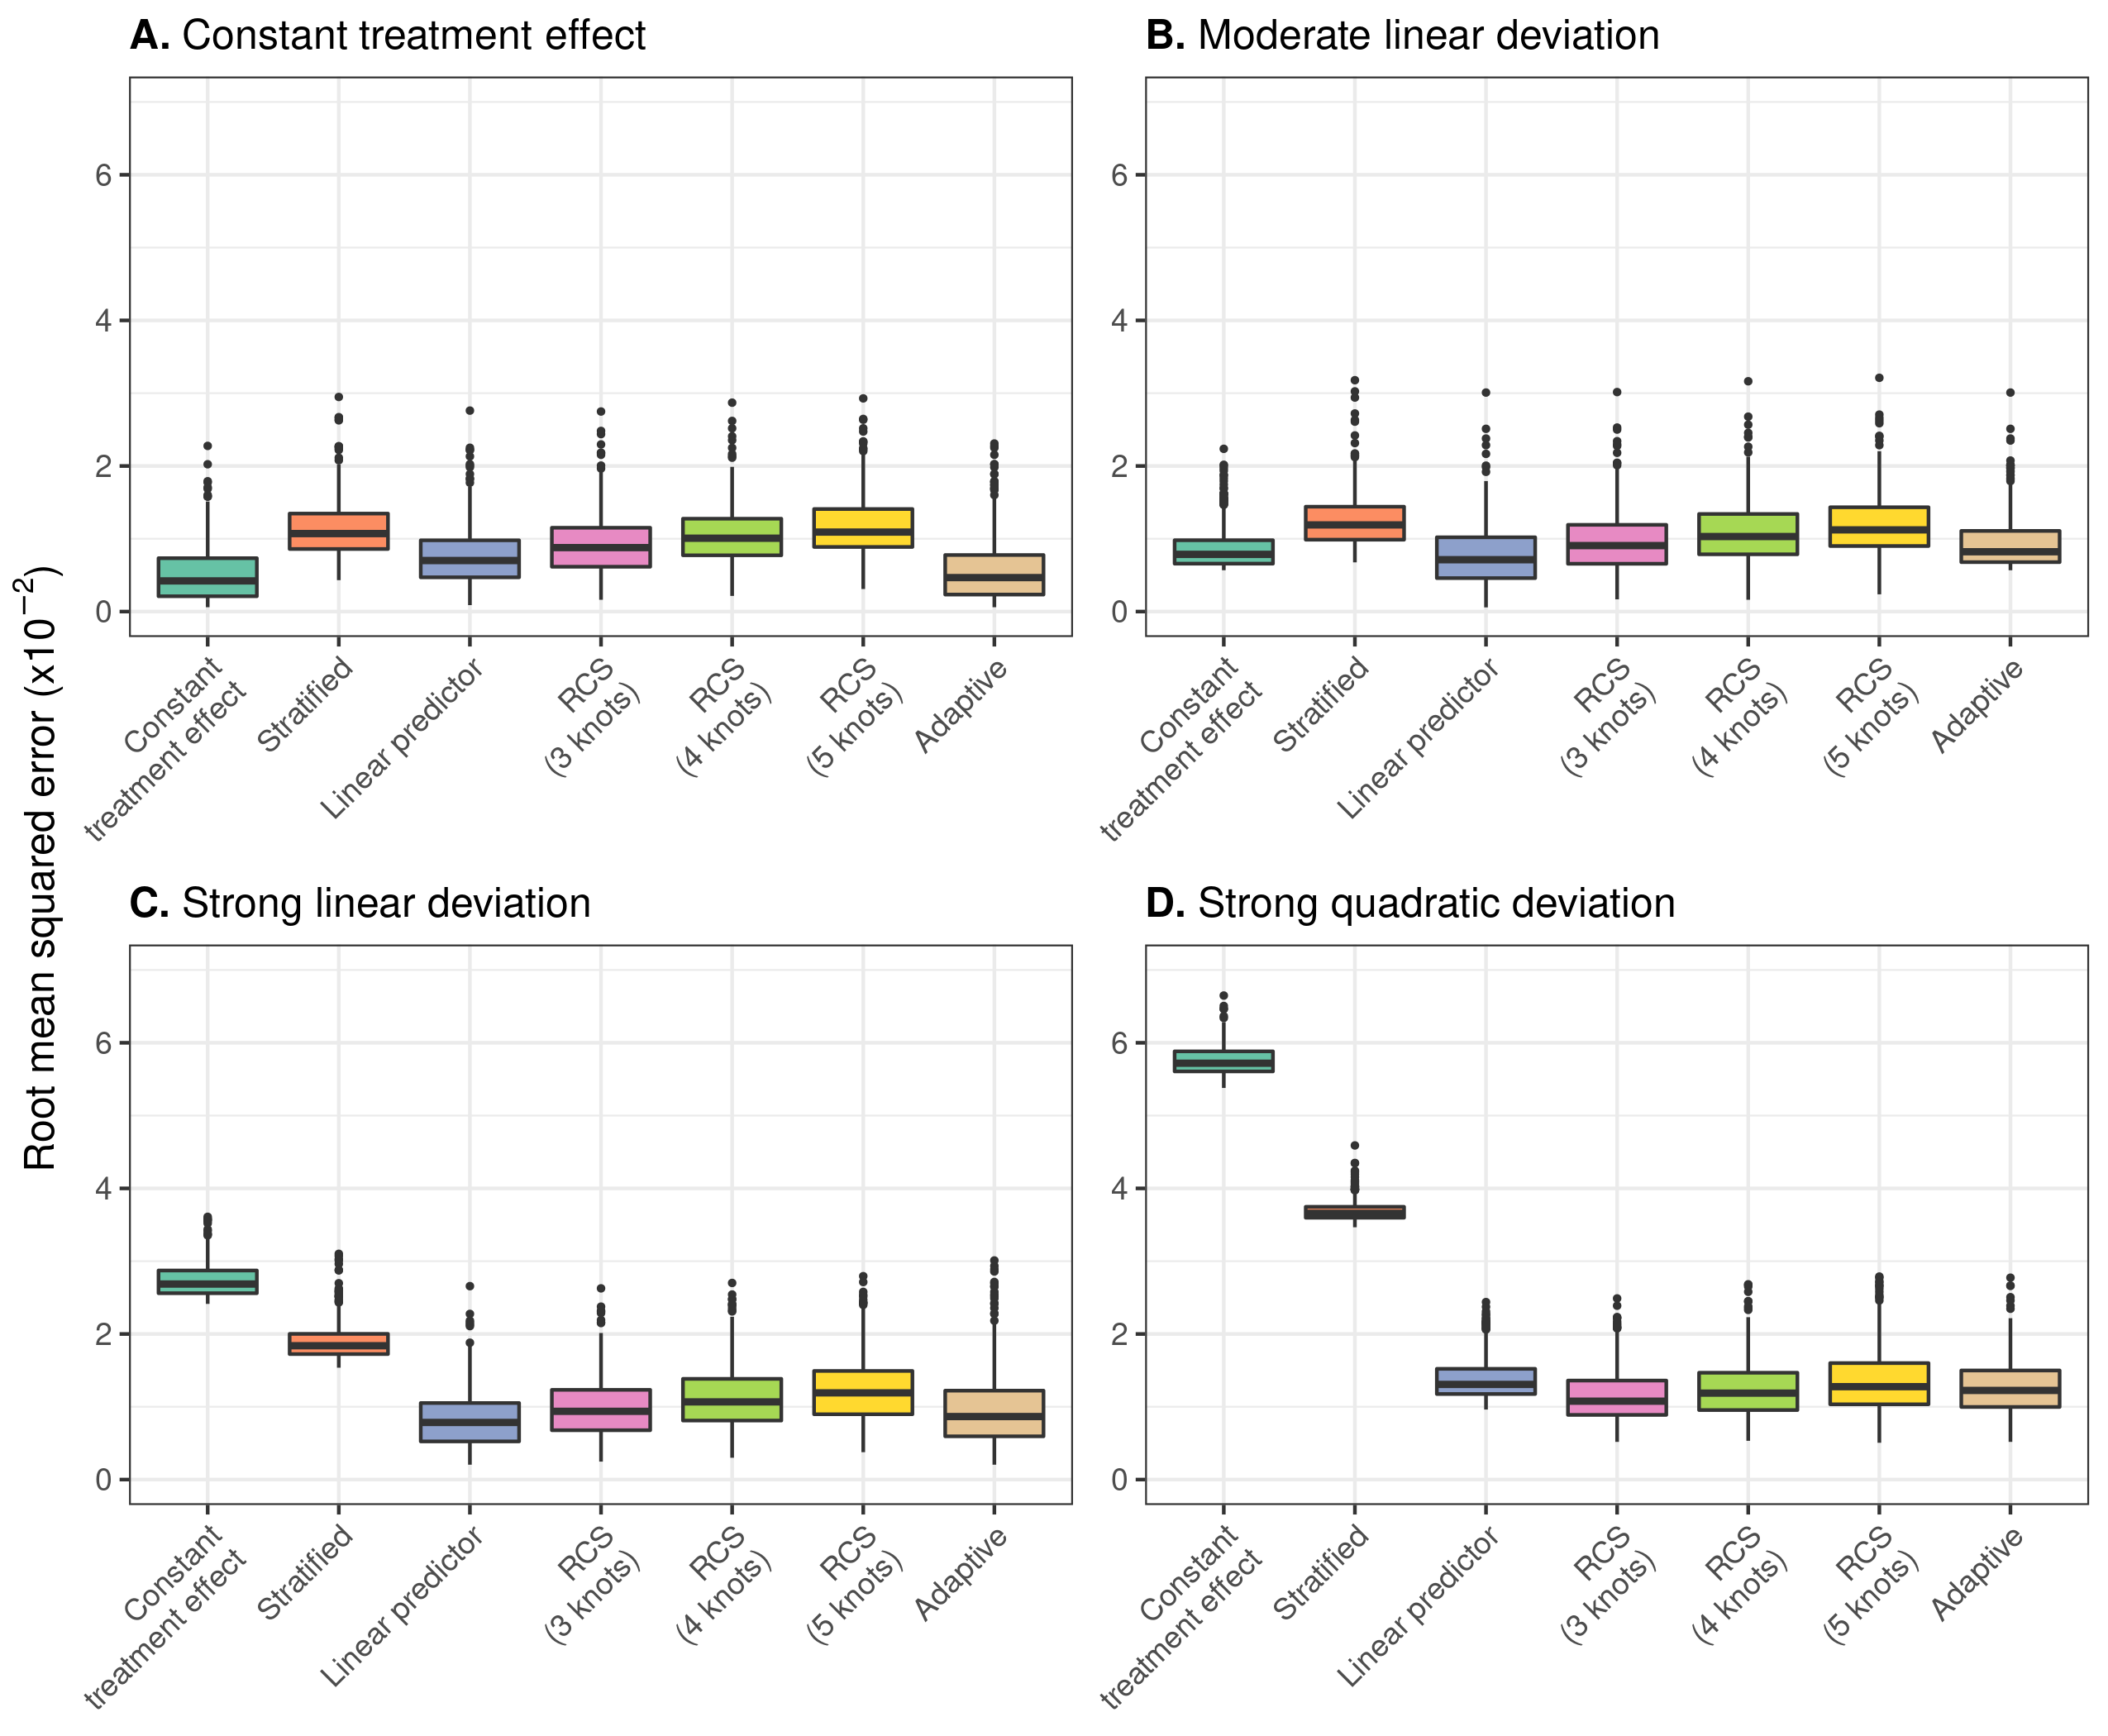
\includegraphics[width=1\linewidth]{/home/arekkas/Documents/Projects/arekkas_HteSimulation_XXXX_2021/figures/rmse_sample_size} \caption{RMSE of the considered methods across 500 replications calculated in a simulated sample of size 500,000. \textit{Panel A} presents the results under the base case scenario of true constant relative treatment effect, with a true prediction AUC of 0.75 and sample size of 17,000; \textit{Panel B} presents the results under moderate linear deviations from constant treatment effects; \textit{Panel C} presents the results for strong linear deviations from constant relative treatment effects; \textit{Panel D} presents the results for strong quadratic deviations constant relative treatment effects.}\label{fig:rmsesamplesize}
\end{figure}

When we increased the true prediction AUC to 0.85, models including RCS
smoothing had the lowest RMSE in the presence of strong quadratic
deviations from the base case of true constant relative treatment
effects (Figure \ref{fig:rmseauc}; Panel D). However, with milder
deviations, the linear interaction model had the lowest RMSE with the
RCS smoothing methods (3 knots) being a close second (Figure
\ref{fig:rmseauc}; Panels B and C). Increasing the number of knots of
RCS smoothing resulted in increased RMSE, which was less pronounced in
the case of strong quadratic deviations.

\begin{figure}
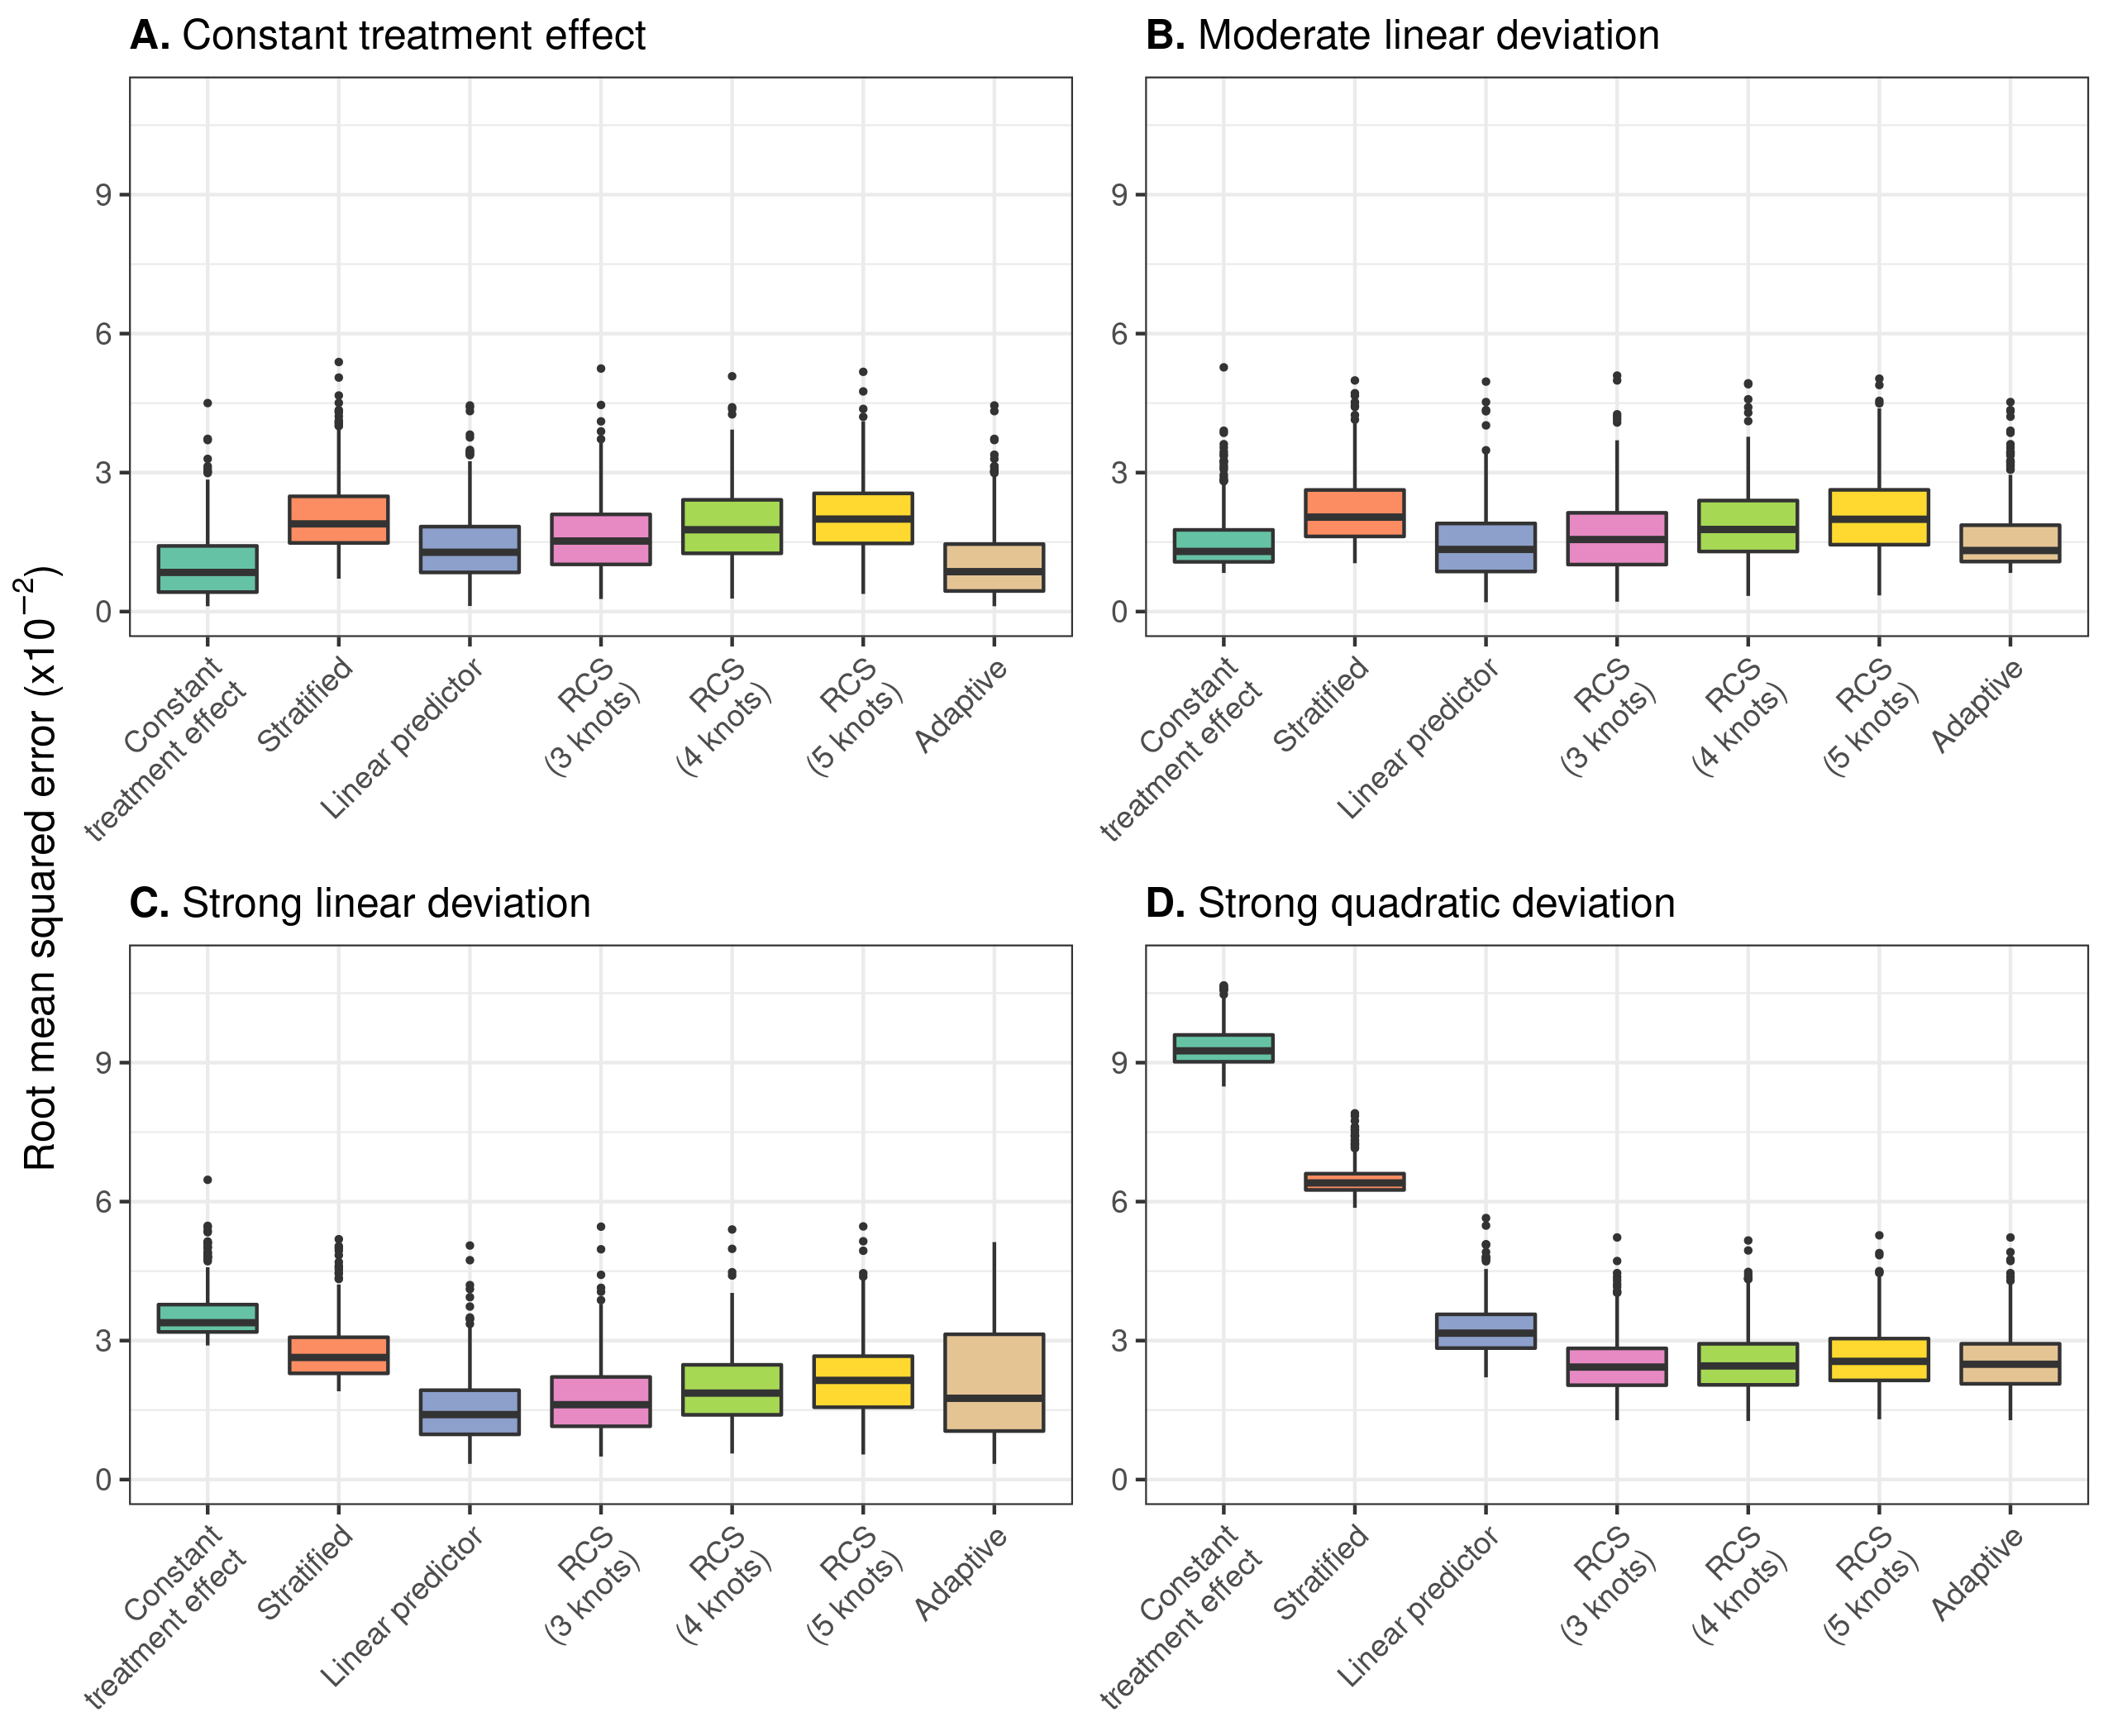
\includegraphics[width=1\linewidth]{/home/arekkas/Documents/Projects/arekkas_HteSimulation_XXXX_2021/figures/rmse_auc} \caption{RMSE of the considered methods across 500 replications calculated in a simulated sample of size 500,000. \textit{Panel A} presents the results under the base case scenario of true constant relative treatment effect, with a true prediction AUC of 0.85 and sample size of 4,250; \textit{Panel B} presents the results under moderate linear deviations from constant treatment effects, while holding true prediction AUC and sample size constant; \textit{Panel C} presents the results for strong linear deviations from constant relative treatment effects; \textit{Panel D} presents the results for strong quadratic deviations from constant relative treatment effects.}\label{fig:rmseauc}
\end{figure}

The constant effects model, the linear interaction model and models with
RCS smoothing (3 knots) had the highest median c-for-benefit in the base
case scenario and the scenarios where linear and quadratic deviations
were considered. The constant treatment effect model and the linear
interaction model tended to present much lower variability compared to
all other approaches (Figure \ref{fig:discrimination}). We also observed
an increasing trend of discrimination for benefit variability and
decreasing median values with increasing number of restricted cubic
spline knots in all scenarios.

\begin{figure}
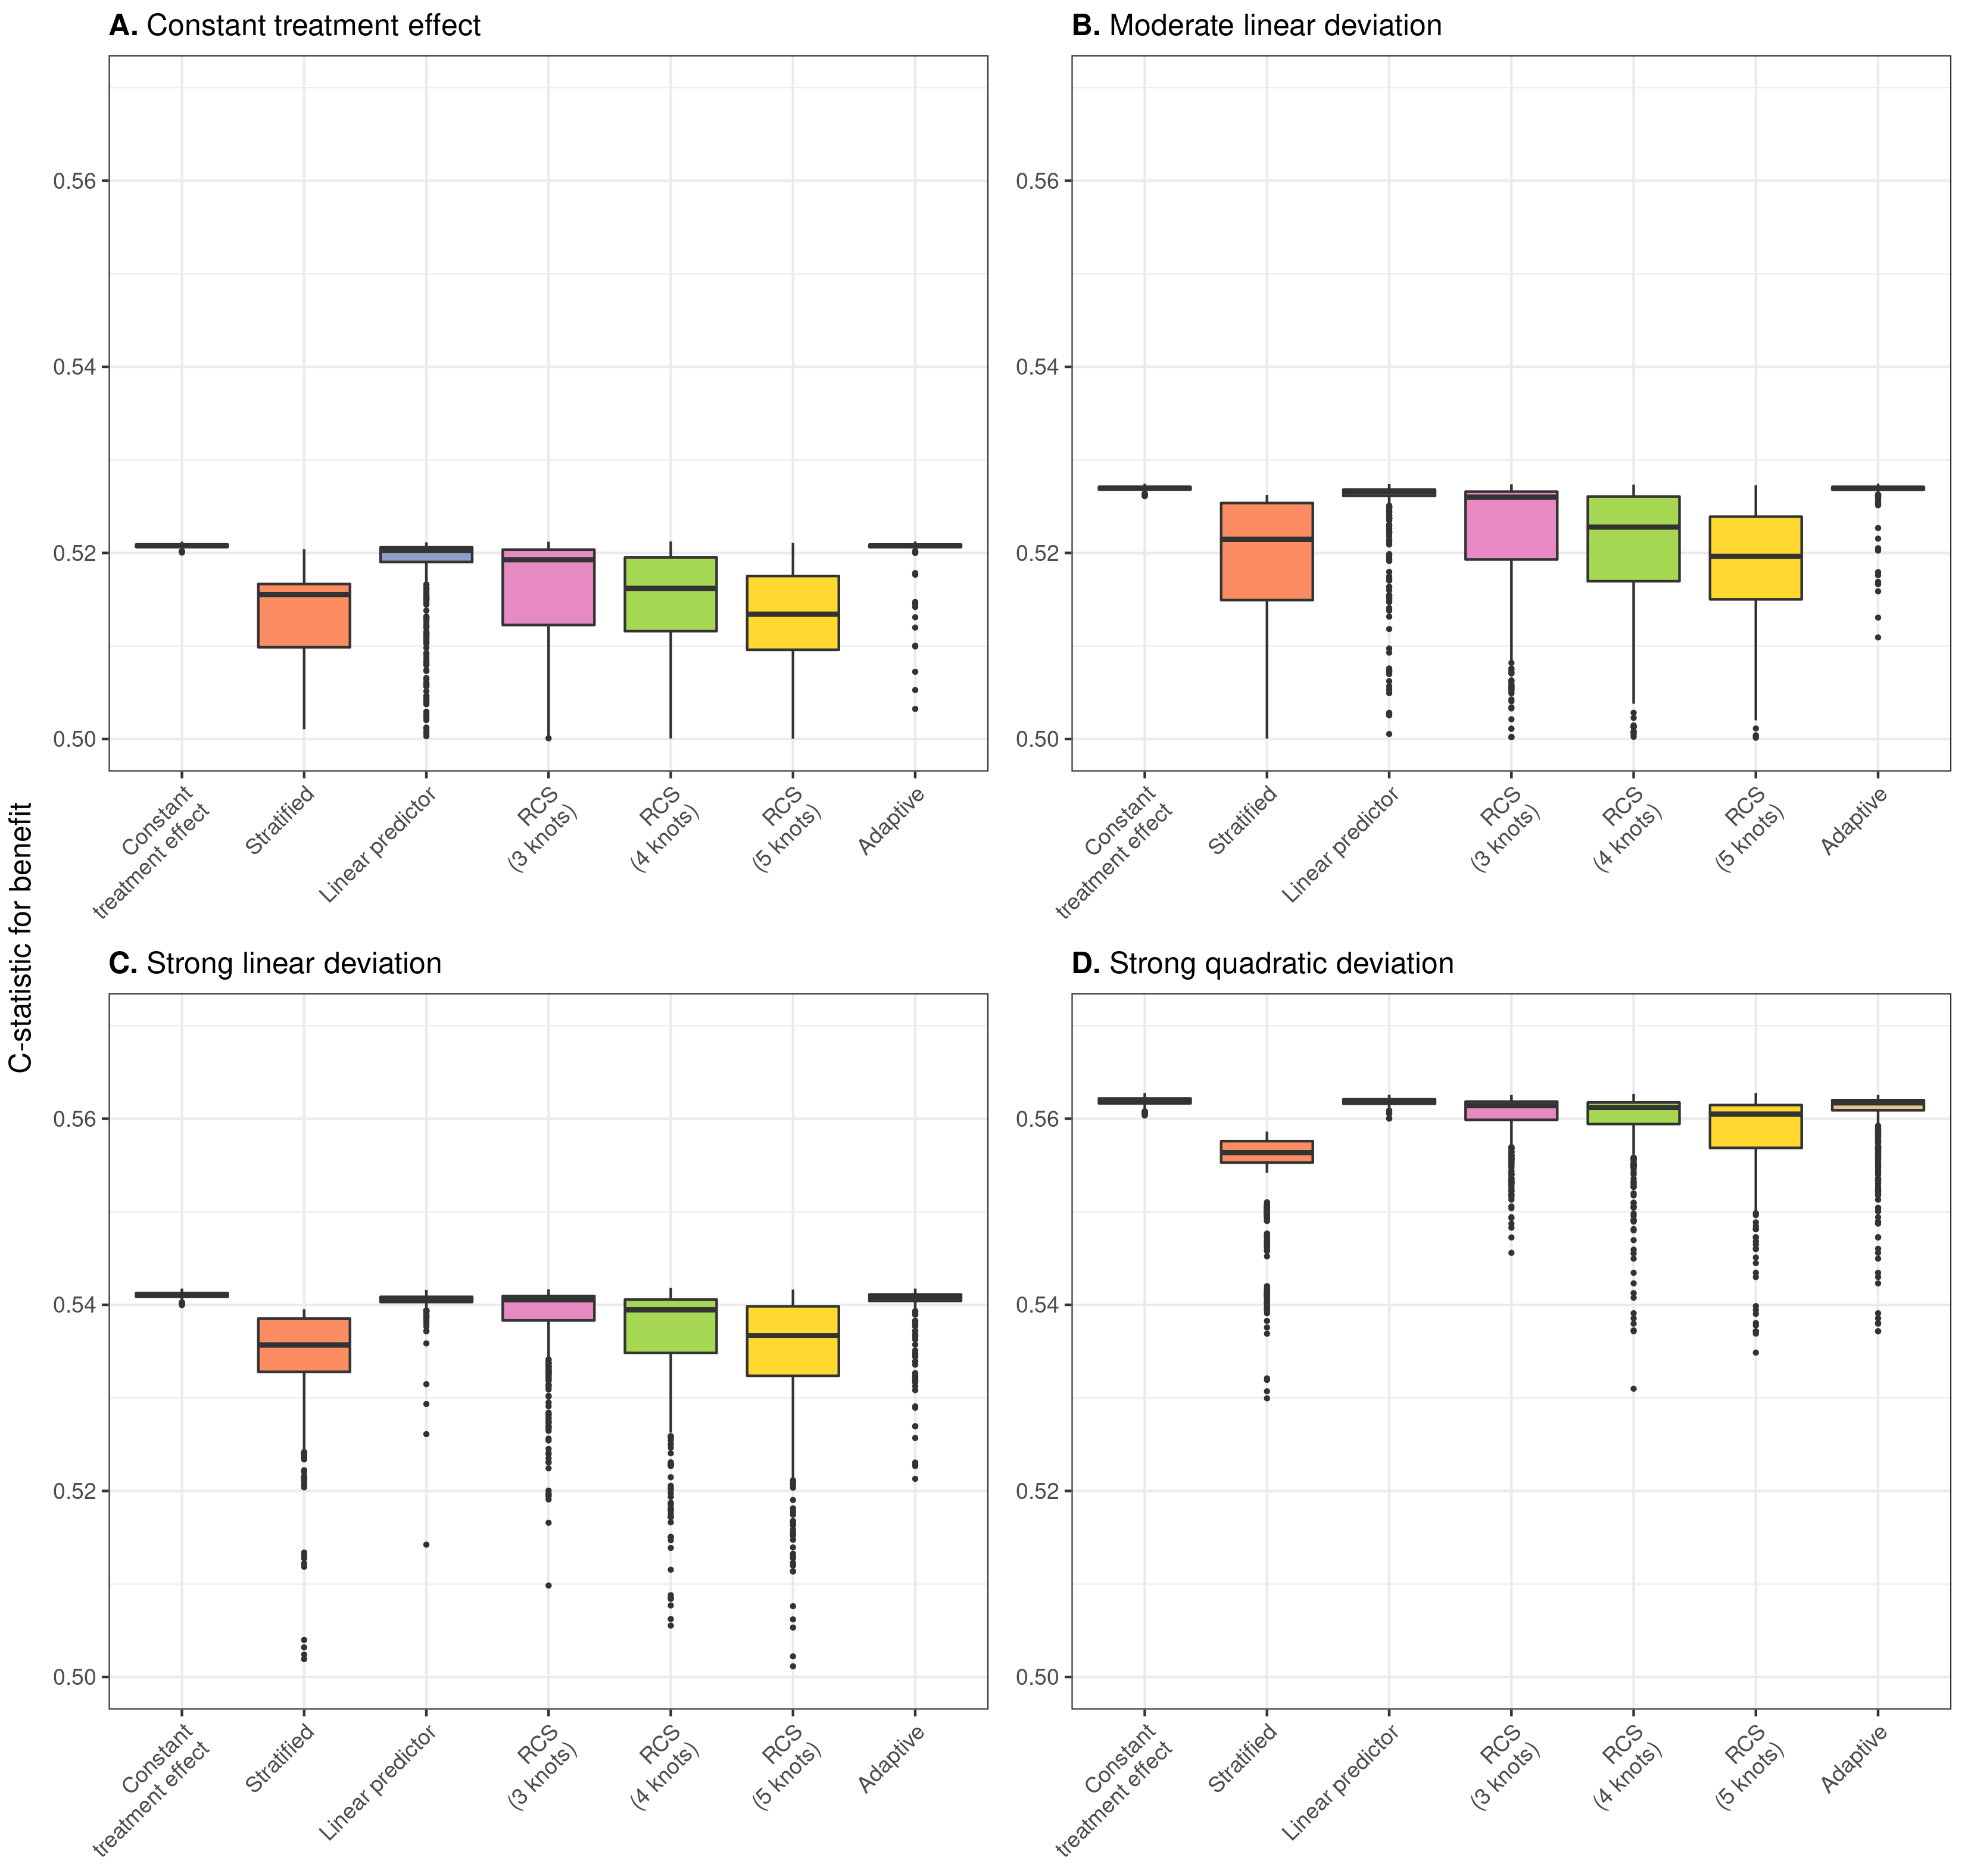
\includegraphics[width=1\linewidth]{/home/arekkas/Documents/Projects/arekkas_HteSimulation_XXXX_2021/figures/discrimination_base} \caption{Discrimination for benefit of the considered methods across 500 replications calculated in a simulated sample of size 500,000. \textit{Panel A} presents the results under the base case scenario of true constant relative treatment effect, with a true prediction AUC of 0.75 and sample size of 4250; \textit{Panel B} presents the results under moderate linear deviations from constant treatment effects; \textit{Panel C} presents the results for strong linear deviations from constant relative treatment effects; \textit{Panel D} presents the results for strong quadratic deviations from constant relative treatment effects.}\label{fig:discrimination}
\end{figure}

When focusing on calibration, the linear interaction model had the
lowest median ICI for benefit in the majority of scenarios except for
the scenarios where no or moderate linear deviations from the base case
were considered. In that case constant treatment effect models
demonstrated the best performance, very comparable to the linear
interaction model's performance, nonetheless (Figure
\ref{fig:calibration}). However, under strong linear or quadratic
deviations, the constant treatment effect model was very poorly
calibrated (Figure \ref{fig:calibration}; Panels C and D).

\begin{figure}
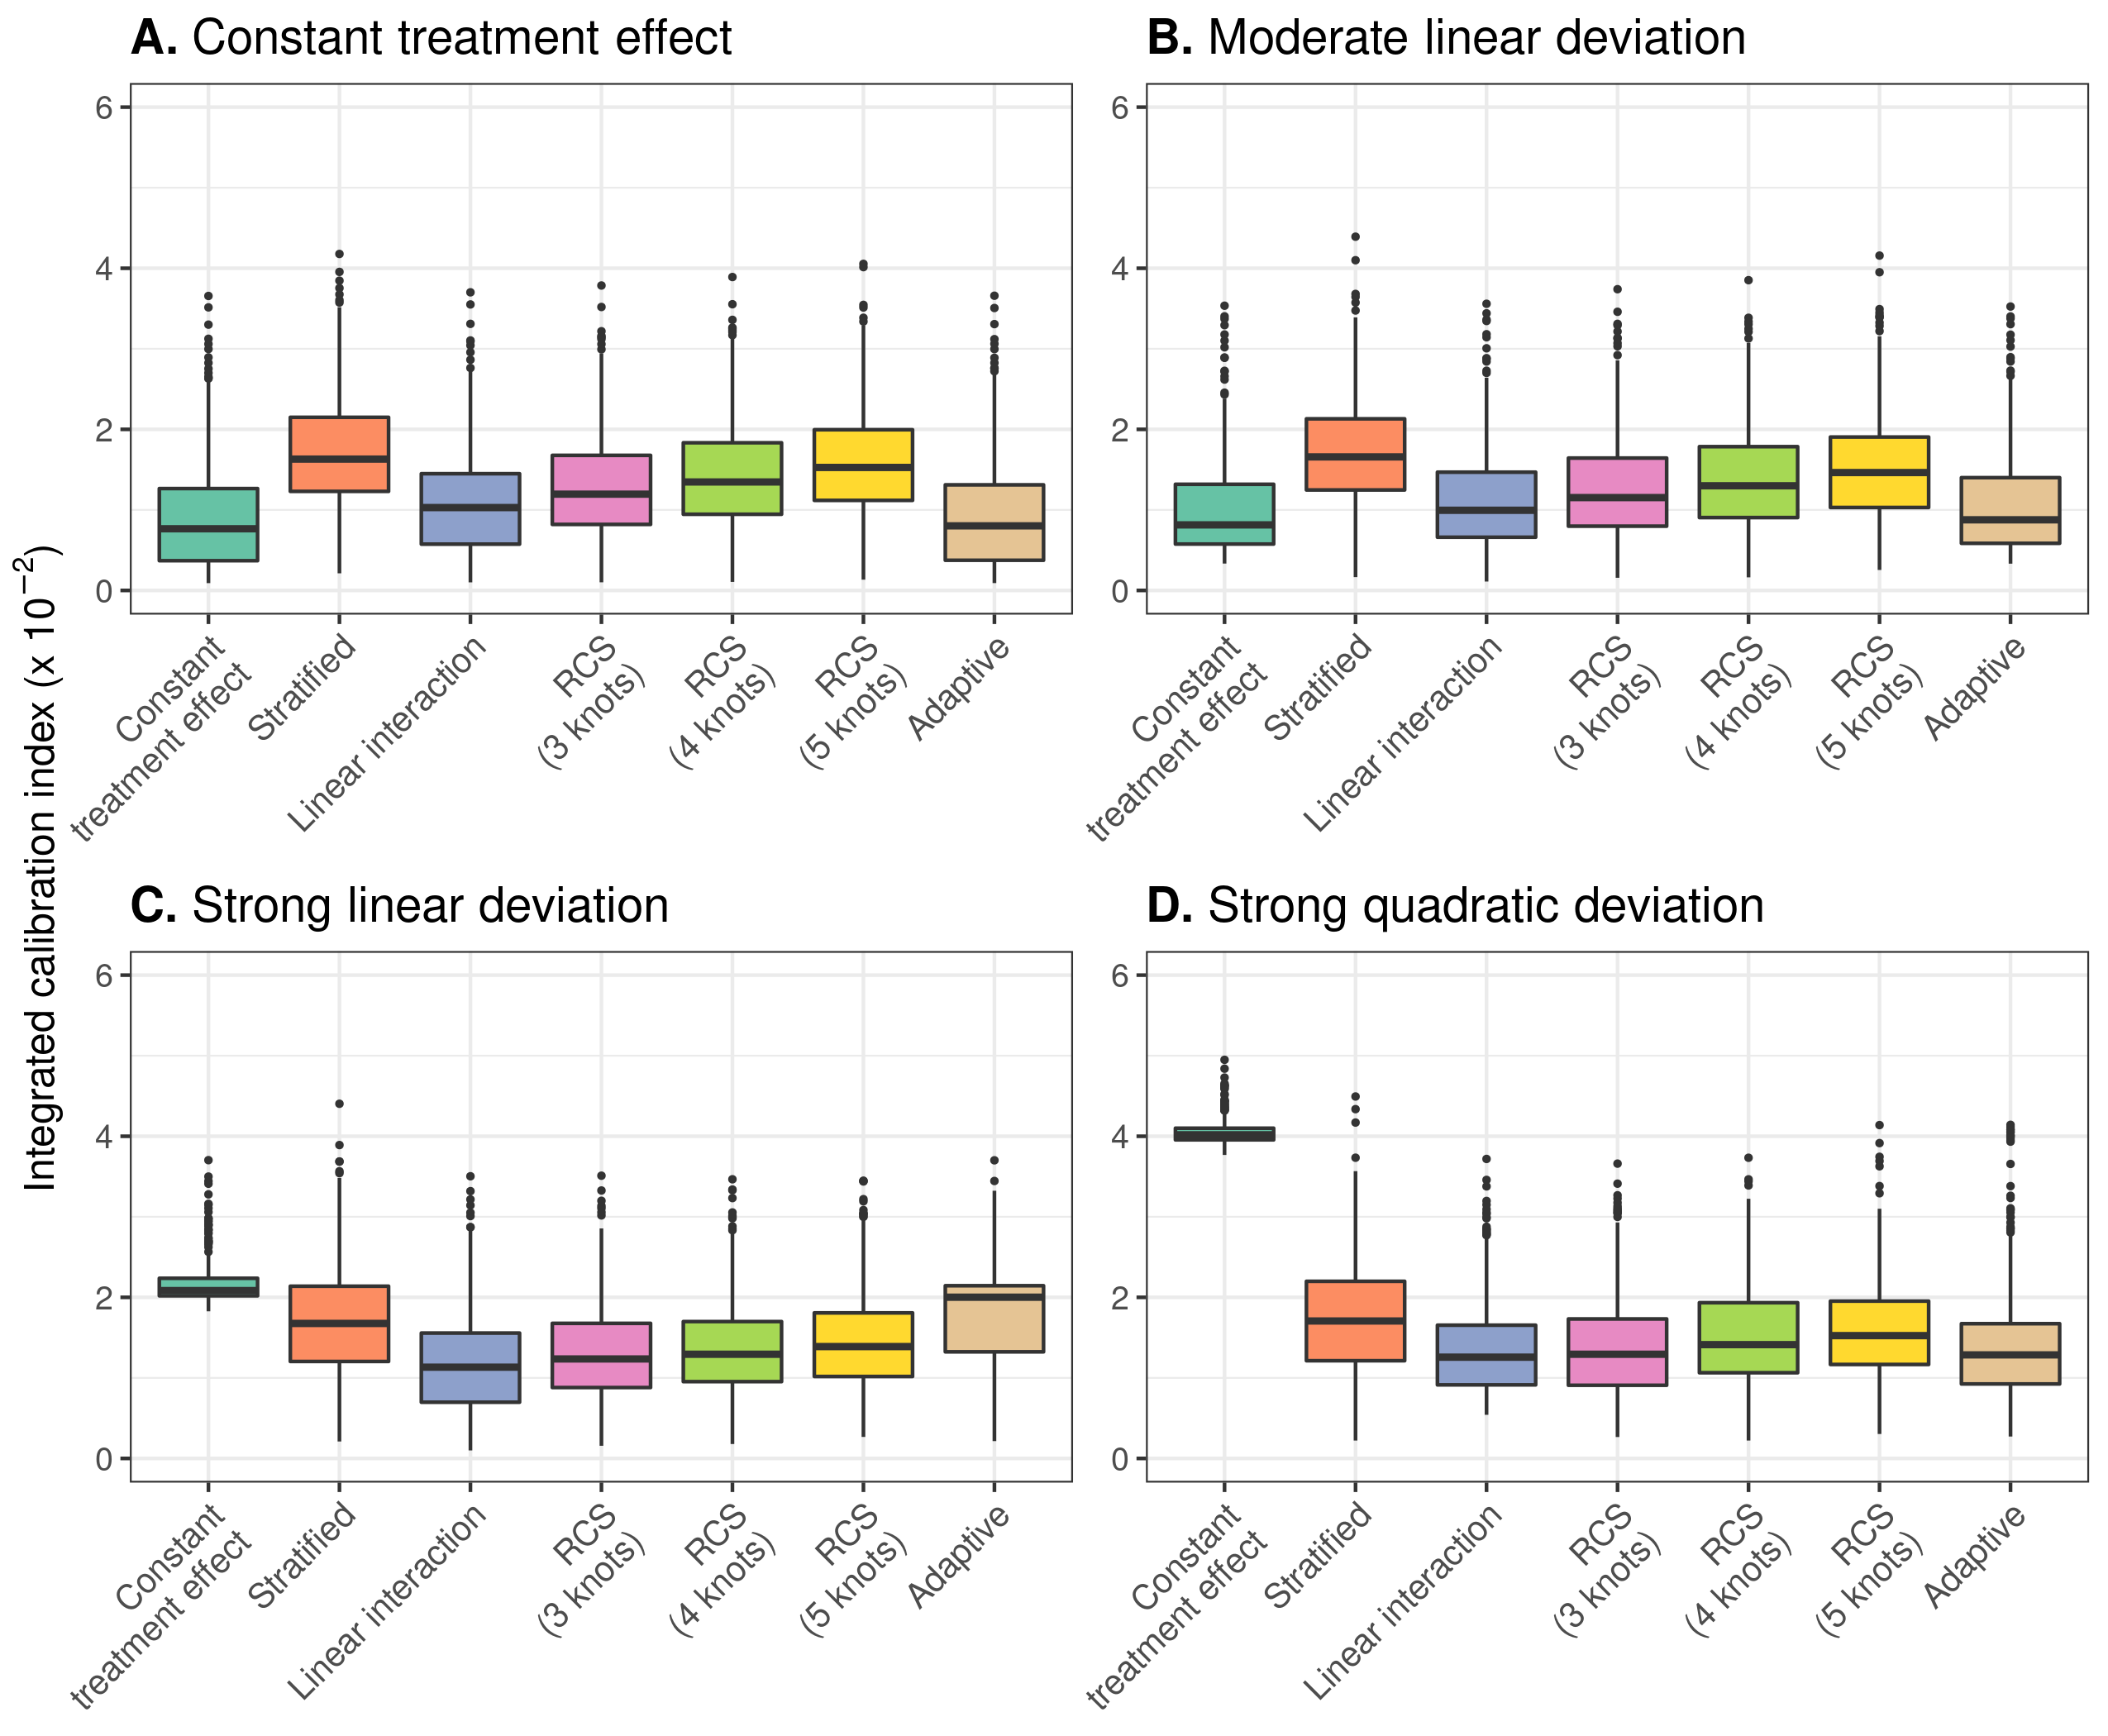
\includegraphics[width=1\linewidth]{/home/arekkas/Documents/Projects/arekkas_HteSimulation_XXXX_2021/figures/calibration_base} \caption{Calibration for benefit of the considered methods across 500 replications calculated in a simulated sample of size 500,000. \textit{Panel A} presents the results under the base case scenario of true constant relative treatment effect, with a true prediction AUC of 0.75 and sample size of 4250; \textit{Panel B} presents the results under moderate linear deviations from constant treatment effectst; \textit{Panel C} presents the results for strong linear deviations from of constant relative treatment effects; \textit{Panel D} presents the results for strong quadratic deviations from constant relative treatment effects.}\label{fig:calibration}
\end{figure}

\hypertarget{case-study}{%
\subsection{Case study}\label{case-study}}

We demonstrate the different methods for individualizing treatment
benefits using data from 30,510 patients with an acute myocardial
infarction (MI) included in the GUSTO-I trial. 10,348 patients were
randomized to tissue plasminogen activator (tPA) treatment and 20,162
were randomized to streptokinase. The outcome of interest was 30-day
mortality, recorded for all patients.

In line with previous analyses {[}10,11{]}, we fitted a logistic
regression model with 6 baseline covariates, i.e.~age, Killip class,
systolic blood pressure, heart rate, an indicator of previous MI, and
the location of MI, to predict 30-day mortality risk. A constant effect
of treatment was included in the model. When deriving risk predictions
for individuals we set the treatment indicator to 0. More information on
model development can be found in the supplement.

We used the risk linear predictor to fit the the proposed methods under
study for individualizing absolute benefit predictions. All methods had
quite comparable results, in the sense that we predicted increasing
benefits for patients with higher baseline risk predictions. In terms of
c-for-benefit (validated internally) all models had quite comparable
performance ranging from 0.519 (RCS smoothing with 3 knots) to 0.542
(RCS smoothing with 4 knots). Similar conclusions could be drawn in
terms of ICI-for-benefit which ranged from 0.0039 (linear interaction
approach) to 0.0053 (RCS smoothing with 4 knots).

The adaptive approach picked the model with RCS smoothing with 4 knots,
which had quite comparable performance to the smooth fit with 5 knots.
However, for lower baseline risk these 2 models predicted implausible
benefits and maybe should be avoided when applying such models in
practice. The linear interaction model and the model with RCS smoothing
(3 knots) made very similar predictions and also followed quite closely
the evolution of the stratified estimates. In this case, we observed
that even using a simple model with a constant relative treatment effect
can result in very similar benefit predictions as other more complex
approaches.

\begin{figure}
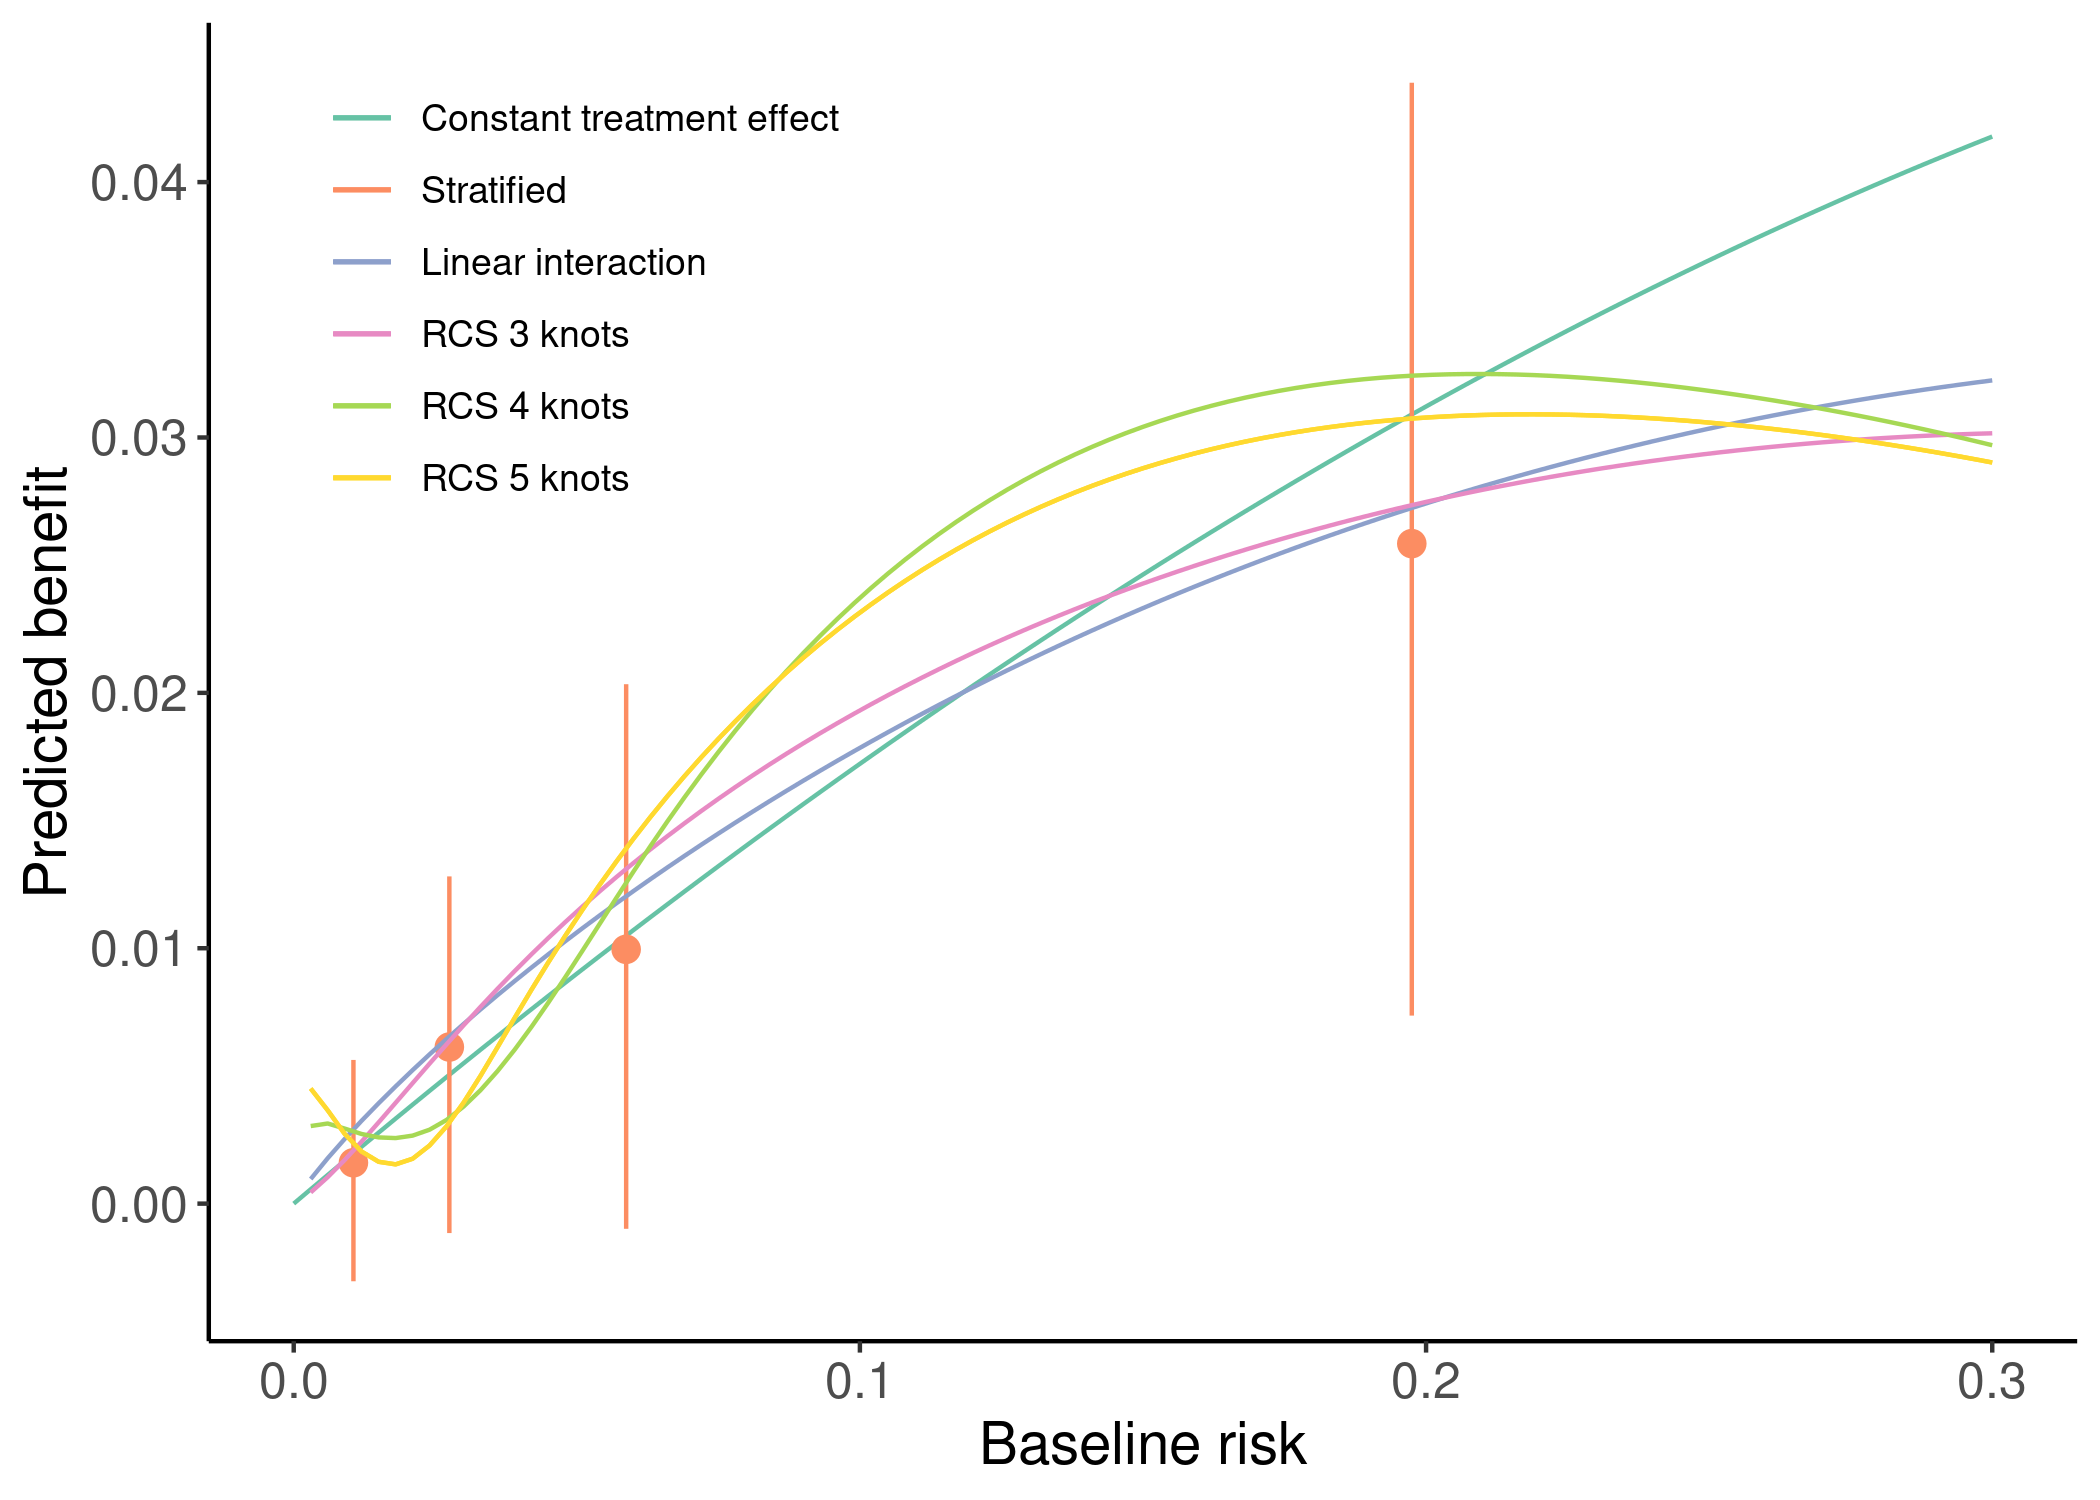
\includegraphics[width=1\linewidth]{/home/arekkas/Documents/Projects/arekkas_HteSimulation_XXXX_2021/figures/gusto} \caption{Individualized absolute benefit predictions based on baseline risk when using a constantn treatment effect approach, a linear interaction approach and RCS smoothing using 3,4 and 5 knots. Risk stratified estimates of absolute benefit are presented within quartiles of baseline risk as reference.}\label{fig:gusto}
\end{figure}

\hypertarget{discussion}{%
\section{Discussion}\label{discussion}}

The linear interaction model proved to be superior to alternative
approaches when predicting risk-based treatment benefit under a wide
range of scenarios. It generally had lower mean squared error, lower
e-for-benefit and higher c-for-benefit with lower variability across
simulation replications. Models including restricted cubic splines with
3 knots only outperformed the linear interaction model in the presence
of strong quadratic deviations from a constant relative treatment
effect.

Including restricted cubic splines with 4 or 5 knots proved to be too
flexible, as indicated by higher RMSE, increased variability of
discrimination for benefit and worse calibration of benefit predictions.
Even with larger sample sizes and strong quadratic deviations from the
base case scenario of constant relative treatment effects, these more
flexible restricted cubic splines did not outperform the simpler RCS
with 3 knots. These more flexible approaches may only be helpful if we
expect more extreme patterns of heterogeneous treatment effects.

The constant treatment effect model, despite having adequate performance
in the presence of weak treatment effect heterogeneity on the relative
scale, quickly broke down with stronger deviations from constant
relative treatment effects. In these cases, the stratified approach
generally had lower error rates compared to the constant treatment
effect model. In concept, the stratified approach lies between the
constant effects model and smoother approaches, only assuming constant
treatment effects within strata of predicted risk and, therefore, is
more sensitive to treatment effect heterogeneity. Stepwise treatment
benefit estimates are very useful for demonstrating treatment effect
heterogeneity -- because estimating treatment effect requires groups of
patients rather than individual patients --but are not helpful for
making individualized absolute benefit predictions.

Increasing the discriminative ability of the risk model -- by increasing
the predictor coefficients of the true risk model -- reduced RMSE for
all methods, similar to increasing the sample size. This increase in
discriminative ability translates in higher variability of predicted
risks, which, in turn, allows the considered methods to better follow
the evolution of treatment benefit. As expected, the increase in
discriminative ability of the risk model also led to higher values of
c-for-benefit. Even though risk model performance is very important for
the ability of risk-based methods to predict treatment benefit,
prediction model development was outside the scope of this work and has
already been studied extensively {[}5,12,13{]}.

Risk-based approaches to predictive HTE estimate treatment benefit as a
function of baseline risk. A limitation of our study is that we assumed
treatment benefit to be a function of baseline risk in the majority of
the simulation scenarios. Nevertheless, our main conclusions did not
change when we generated individual treatment-covariate interactions
(supplementary table/figure x). Future simulation studies could explore
the effect of more extensive deviations from risk-based treatment
effects.

Recent years have seen an increased interest in predictive HTE
approaches focusing on individualized benefit predictions. In our
simulations we only focused on risk-based methods, using baseline risk
as a reference in a two-stage approach to individualizing benefit
predictions. However, there is a plethora of different methods, ranging
from treatment effect modeling to tree-based approaches available in
more recent literature {[}14--16{]}. Simulations are also needed to
assess relative performance and define the settings where these break
down or outperform each other.

In conclusion, when comparing different risk-based approaches to predict
individualizing benefit a models including a linear treatment
interaction with the prognostic performed best in a wide range of
scenarios. More flexible models with restricted cubic splines required
larger sample sizes and higher AUC of the PI to outperform the linear
model. An adaptive approach, selecting the model with optimal AIC, had
satisfactory performance.

\newpage

\hypertarget{references}{%
\section{References}\label{references}}

\nolinenumbers
\setlength{\parindent}{-0.25in}
\setlength{\leftskip}{0.25in}

\noindent

\hypertarget{refs}{}
\begin{cslreferences}
\leavevmode\hypertarget{ref-Varadhan2013}{}%
{[}1{]} Varadhan R, Segal JB, Boyd CM, Wu AW, Weiss CO. A framework for
the analysis of heterogeneity of treatment effect in~patient-centered
outcomes research. Journal of Clinical Epidemiology 2013;66:818--25.
\url{https://doi.org/10.1016/j.jclinepi.2013.02.009}.

\leavevmode\hypertarget{ref-Rekkas2020}{}%
{[}2{]} Rekkas A, Paulus JK, Raman G, Wong JB, Steyerberg EW, Rijnbeek
PR, et al. Predictive approaches to heterogeneous treatment effects: A
scoping review. BMC Medical Research Methodology 2020;20.
\url{https://doi.org/10.1186/s12874-020-01145-1}.

\leavevmode\hypertarget{ref-Kent2019}{}%
{[}3{]} Kent DM, Paulus JK, Klaveren D van, D'Agostino R, Goodman S,
Hayward R, et al. The predictive approaches to treatment effect
heterogeneity (PATH) statement. Annals of Internal Medicine 2019;172:35.
\url{https://doi.org/10.7326/m18-3667}.

\leavevmode\hypertarget{ref-PathEnE}{}%
{[}4{]} Kent DM, Klaveren D van, Paulus JK, D'Agostino R, Goodman S,
Hayward R, et al. The predictive approaches to treatment effect
heterogeneity (PATH) statement: Explanation and elaboration. Annals of
Internal Medicine 2019;172:W1. \url{https://doi.org/10.7326/m18-3668}.

\leavevmode\hypertarget{ref-vanKlaveren2019}{}%
{[}5{]} Klaveren D van, Balan TA, Steyerberg EW, Kent DM. Models with
interactions overestimated heterogeneity of treatment effects and were
prone to treatment mistargeting. Journal of Clinical Epidemiology
2019;114:72--83. \url{https://doi.org/10.1016/j.jclinepi.2019.05.029}.

\leavevmode\hypertarget{ref-Kent2010}{}%
{[}6{]} Kent DM, Rothwell PM, Ioannidis JP, Altman DG, Hayward RA.
Assessing and reporting heterogeneity in treatment effects in clinical
trials: A proposal. Trials 2010;11.
\url{https://doi.org/10.1186/1745-6215-11-85}.

\leavevmode\hypertarget{ref-Harrell1988}{}%
{[}7{]} Harrell FE, Lee KL, Pollock BG. Regression models in clinical
studies: Determining relationships between predictors and response. JNCI
Journal of the National Cancer Institute 1988;80:1198--202.
\url{https://doi.org/10.1093/jnci/80.15.1198}.

\leavevmode\hypertarget{ref-vanKlaveren2018}{}%
{[}8{]} Klaveren D van, Steyerberg EW, Serruys PW, Kent DM. The proposed
``concordance-statistic for benefit'' provided a useful metric when
modeling heterogeneous treatment effects. Journal of Clinical
Epidemiology 2018;94:59--68.
\url{https://doi.org/10.1016/j.jclinepi.2017.10.021}.

\leavevmode\hypertarget{ref-Austin2019}{}%
{[}9{]} Austin PC, Steyerberg EW. The integrated calibration index (ICI)
and related metrics for quantifying the calibration of logistic
regression models. Statistics in Medicine 2019;38:4051--65.
\url{https://doi.org/10.1002/sim.8281}.

\leavevmode\hypertarget{ref-Califf1997}{}%
{[}10{]} Califf RM, Woodlief LH, Harrell FE, Lee KL, White HD, Guerci A,
et al. Selection of thrombolytic therapy for individual patients:
Development of a clinical model. American Heart Journal 1997;133:630--9.
\url{https://doi.org/10.1016/s0002-8703(97)70164-9}.

\leavevmode\hypertarget{ref-Steyerberg2000}{}%
{[}11{]} Steyerberg EW, Bossuyt PMM, Lee KL. Clinical trials in acute
myocardial infarction: Should we adjust for baseline characteristics?
American Heart Journal 2000;139:745--51.
\url{https://doi.org/10.1016/s0002-8703(00)90001-2}.

\leavevmode\hypertarget{ref-Burke2014}{}%
{[}12{]} Burke JF, Hayward RA, Nelson JP, Kent DM. Using internally
developed risk models to assess heterogeneity in treatment effects in
clinical trials. Circulation: Cardiovascular Quality and Outcomes
2014;7:163--9. \url{https://doi.org/10.1161/circoutcomes.113.000497}.

\leavevmode\hypertarget{ref-Abadie2018}{}%
{[}13{]} Abadie A, Chingos MM, West MR. Endogenous stratification in
randomized experiments. The Review of Economics and Statistics
2018;100:567--80. \url{https://doi.org/10.1162/rest_a_00732}.

\leavevmode\hypertarget{ref-Athey2019}{}%
{[}14{]} Athey S, Tibshirani J, Wager S. Generalized random forests. The
Annals of Statistics 2019;47. \url{https://doi.org/10.1214/18-aos1709}.

\leavevmode\hypertarget{ref-Lu2018}{}%
{[}15{]} Lu M, Sadiq S, Feaster DJ, Ishwaran H. Estimating individual
treatment effect in observational data using random forest methods.
Journal of Computational and Graphical Statistics 2018;27:209--19.
\url{https://doi.org/10.1080/10618600.2017.1356325}.

\leavevmode\hypertarget{ref-Wager2018}{}%
{[}16{]} Wager S, Athey S. Estimation and inference of heterogeneous
treatment effects using random forests. Journal of the American
Statistical Association 2018;113:1228--42.
\url{https://doi.org/10.1080/01621459.2017.1319839}.
\end{cslreferences}

\setlength{\parindent}{0in}
\setlength{\leftskip}{0in}

\noindent

\bibliographystyle{unsrt}
\bibliography{references.bib}


\end{document}
